\documentclass[10pt]{article}
\usepackage[ruled, linesnumbered]{algorithm2e}
\usepackage{Jan1, epsfig, subfigure, amssymb, multirow, algorithmic,amsmath}
\usepackage{latexsym,amssymb,epsfig,graphicx,subfigure,rotating,multirow,colortbl,xcolor,amsmath,algorithmic,booktabs,url}
\usepackage{accents}
\usepackage{subfig}
\textwidth 160mm
\textheight 215mm
\voffset 1mm
\oddsidemargin 1mm
\evensidemargin 1mm
\newtheorem{definition}{Definition}
\newtheorem{theorem}{Theorem}
\newtheorem{proposition}{Proposition}
\newtheorem{conjecture}{Conjecture}
\newtheorem{corollary}{Corollary}
\newtheorem{lemma}{Lemma}
\newtheorem{example}{Example}


\usepackage[english]{babel}
\usepackage{blindtext}


\title{VHM simulation with {\sf Cpp}-runtime in OpenModelica}

\author{Anton de Villiers\thanks{HealthQ Technologies, Office 9, First Floor, The Woodmill Lifestyle, Vredenburg Road, Devon Valley,
Stellenbosch, 7600, South Africa}}

\renewcommand{\thefigure}{\arabic{section}.\arabic{figure}}
\renewcommand{\thetable}{\arabic{section}.\arabic{table}}
\begin{document}
\setcounter{page}{1}



\newcommand{\blokkie}{\hspace{.07cm}\Box\hspace{.07cm}}

%%%%% Set up the coloured tables %%%%%
\colorlet{tableheadcolor}{gray!25} % Table header colour = 25% gray
\colorlet{tablerowcolor}{gray!10} % Table row separator colour = 10% gray
\newcommand{\headcol}{\rowcolor{tableheadcolor}}
\newcommand{\rowcol}{\rowcolor{tablerowcolor}}

% The top-most line of a table
\newcommand{\topline}{\arrayrulecolor{black}\specialrule{0.1em}{\abovetopsep}{0pt}%
	\arrayrulecolor{tableheadcolor}\specialrule{\belowrulesep}{0pt}{0pt}%
	\arrayrulecolor{black}}

	% The top-most line of a table
\newcommand{\toplinee}{\arrayrulecolor{black}\specialrule{0.1em}{\abovetopsep}{0pt}%
	\arrayrulecolor{tablerowcolor}\specialrule{\belowrulesep}{0pt}{0pt}%
	\arrayrulecolor{black}}

% The line between the headings and the table body
\newcommand{\midline}{\arrayrulecolor{tableheadcolor}\specialrule{\aboverulesep}{0pt}{0pt}%
	\arrayrulecolor{black}\specialrule{\lightrulewidth}{0pt}{0pt}%
	\arrayrulecolor{white}\specialrule{\belowrulesep}{0pt}{0pt}%
	\arrayrulecolor{black}}

% A line for when the upper row is rowcolor and the next line is white
\newcommand{\midlinecbw}{\arrayrulecolor{tablerowcolor}\specialrule{\aboverulesep}{0pt}{0pt}%
	\arrayrulecolor{black}\specialrule{\lightrulewidth}{0pt}{0pt}%
 	\arrayrulecolor{white}\specialrule{\belowrulesep}{0pt}{0pt}%
	\arrayrulecolor{black}}

% A line with no black, to further separate a rowcolor row and a white row
\newcommand{\midlinecw}{\arrayrulecolor{tablerowcolor}\specialrule{\aboverulesep}{0pt}{0pt}%
	\arrayrulecolor{tablerowcolor}\specialrule{\lightrulewidth}{0pt}{0pt}%
	\arrayrulecolor{white}\specialrule{\belowrulesep}{0pt}{0pt}%
	\arrayrulecolor{black}}

% A line for when the upper row is white and the next line is rowcolor
\newcommand{\midlinewbc}{\arrayrulecolor{white}\specialrule{\aboverulesep}{0pt}{0pt}%
	\arrayrulecolor{black}\specialrule{\lightrulewidth}{0pt}{0pt}%
	\arrayrulecolor{tablerowcolor}\specialrule{\belowrulesep}{0pt}{0pt}%
	\arrayrulecolor{black}}

% sadfsdfsdf sdfsdfsdf
\newcommand{\midlinehr}{\arrayrulecolor{tablerowcolor}\specialrule{\aboverulesep}{0pt}{0pt}%
	\arrayrulecolor{black}\specialrule{\lightrulewidth}{0pt}{0pt}%
	\arrayrulecolor{tableheadcolor}\specialrule{\belowrulesep}{0pt}{0pt}%
	\arrayrulecolor{tablerowcolor}}


% A line for the bottom of the table, when the last row is white
\newcommand{\bottomline}{\arrayrulecolor{white}\specialrule{\aboverulesep}{0pt}{0pt}%
	\arrayrulecolor{black}\specialrule{\heavyrulewidth}{0pt}{\belowbottomsep}}%

% A line for the bottom of the table, when the last row is rowcolor
\newcommand{\bottomlinec}{\arrayrulecolor{tablerowcolor}\specialrule{\aboverulesep}{0pt}{0pt}%
	\arrayrulecolor{black}\specialrule{\heavyrulewidth}{0pt}{\belowbottomsep}}%

\newcommand{\bottomlinect}{\arrayrulecolor{tableheadcolor}\specialrule{\aboverulesep}{0pt}{0pt}%
	\arrayrulecolor{black}\specialrule{\heavyrulewidth}{0pt}{\belowbottomsep}}%
%%%%% Set up the coloured tables %%%%%



\maketitle



\pagestyle{myheadings}


\section{Introduciton}

Franke {\em et al.}~\cite{CppRuntime} investigated the exploitation of {\sf Cpp} ({\sf C++}) for Modelica code optimization. They claim that ``a publically available application example demonstrates the achievements. CPU times obtained with the OpenModelica~\cite{OpenModelica} C++ runtime are significantly faster than CPU times obtained with the C runtime or with Dymola.''

We therefore decided to investigate this claim by focusing on the VHM. The first steps involve building OpenModelica with the {\tt{CppRuntime}} flag enabled.

\section{Results}

Some preliminary numerical tests were performed with the following parameters:
\begin{itemize}
 \item stopTime = {\sf 100}
 \item tolerance = {\sf 1e-6}
 \item numberOfIntervals = {\sf 500}
\end{itemize}

We investigated the DASSL solver with the {\sf C} runtime. For the {\sf C++} runtime, we investigated the following solvers:
\begin{itemize}
 \item DASSL
 \item CVode
 \item IDA
\end{itemize}

An Intel(R) Core(TM) i7-4710MQ CPU @ 2.50GHz computer containing 8 processors and 16GB RAM, using operating system Linux Ubuntu 14.04 was used for the tests.

Graphical results are shown in Figure~\ref{Fig:1} and Figure~\ref{Fig:2}.

A breakdown of the execution times are provided in Table~\ref{Tab:1}. Notice that the compilation times are larger for the {\sf C++} runs as opposed to the {\sf C} run, but the simulation times are shorter for the {\sf C++} runs. The DASSL and CVode solvers seem to provide the quickest execution times for the VHM in {\sf C++} runtime.

\begin{table}[htbp]
	\centering
		\begin{tabular}{cccrccccc}
    \topline	\headcol
   Runtime& Solver & \multicolumn{2}{c}{Times} \\\midline
  && timeFrontend & 1.605435356\\
  &&  timeBackend & 2.04504742\\
   && timeSimCode & 0.328685344\\
   {\sf C} & DASSL &  timeTemplates & 0.799143101\\
   && timeCompile & 5.007660417\\
   && timeSimulation & 31.422863225\\
   && timeTotal & 41.208929966\\ \rowcol
   && timeFrontend& 1.505189705\\\rowcol
  &&  timeBackend &1.982867962\\\rowcol
   && timeSimCode & 0.3326616499\\\rowcol
   {\sf C++} & DASSL &  timeTemplates & 2.469315036\\\rowcol
  &&  timeCompile & 21.191103299\\\rowcol
  &&  timeSimulation & 4.864816006\\\rowcol
  &&  timeTotal & 32.346041009\\
   && timeFrontend & 1.521981099\\
   && timeBackend & 1.997048266\\
   && timeSimCode & 0.320210118\\
   {\sf C++} & CVode &  timeTemplates & 2.463317947\\
  &&  timeCompile & 21.14042106\\
  &&  timeSimulation & 4.865331074\\
  &&  timeTotal & 32.308397227\\\rowcol
  &&      timeFrontend & 1.513984494\\\rowcol
  && timeBackend & 1.993646609\\\rowcol
   && timeSimCode & 0.33445055699\\\rowcol
   {\sf C++} & IDA &  timeTemplates & 2.501393176\\\rowcol
  &&  timeCompile & 21.10962507\\\rowcol
 &&   timeSimulation & 13.587780533\\\rowcol
 &&   timeTotal & 41.040962892\\\bottomlinec
    \end{tabular}
    \caption{Simulation times in seconds.}\label{Tab:1}
    \end{table}

\begin{figure}[htbp]
\begin{center}
\begin{tabular}{cc}
		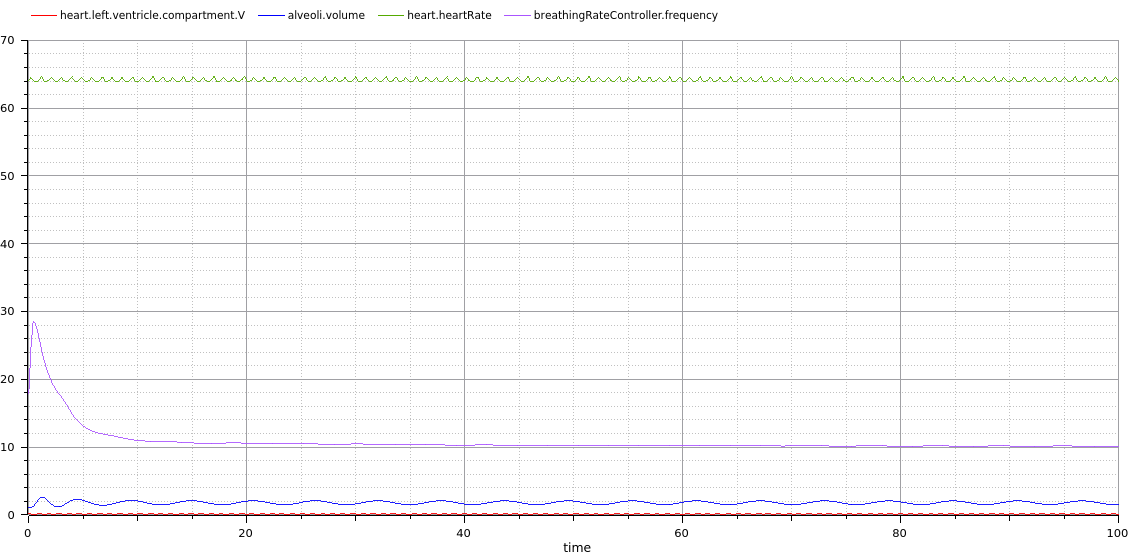
\includegraphics[scale=0.45]{DasslC.png}		\\
		\footnotesize(a) {\sf C} compilation code using DASSL	\\
			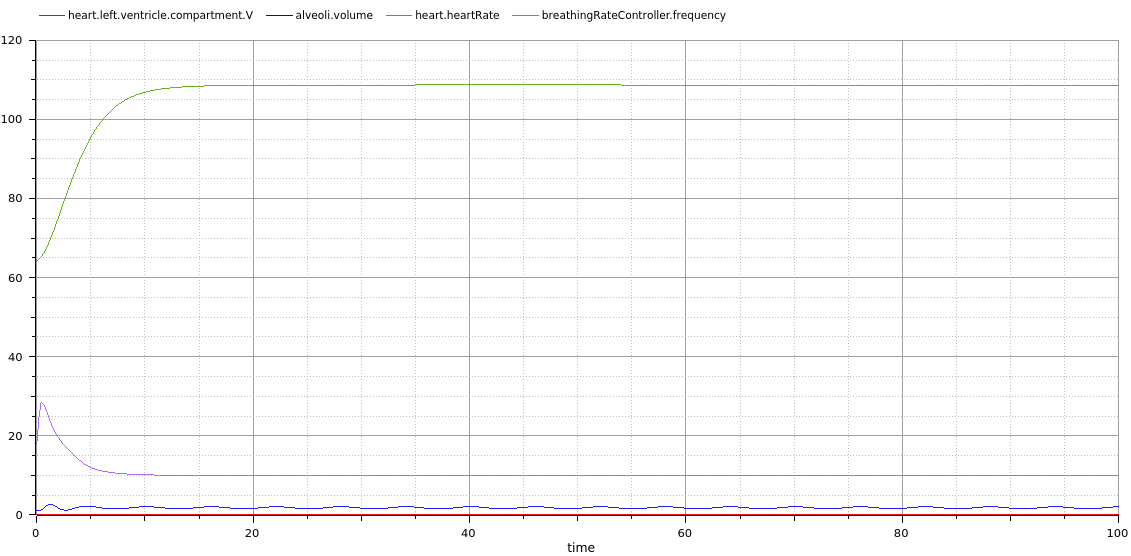
\includegraphics[scale=0.45]{DasslCpp.png}\\
			\footnotesize(b) {\sf C++} compilation code using DASSL\\
	\end{tabular}
\end{center}
\vspace{-0.5cm}

\caption{Numerical results of the DASSL solvers in (a) {\sf C} and (b) {\sf C++} for the VHM.} \label{Fig:1}
\end{figure}

\begin{figure}[htbp]
\begin{center}
\begin{tabular}{cc}
		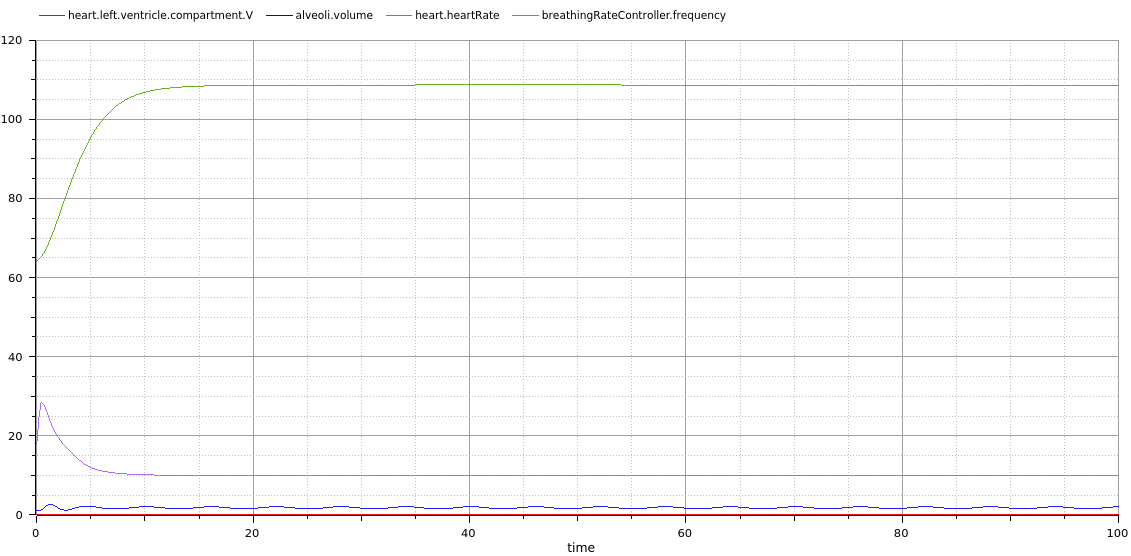
\includegraphics[scale=0.45]{CVodeCpp.png}		\\
		\footnotesize(a) {\sf C++} compilation code using CVode	\\
			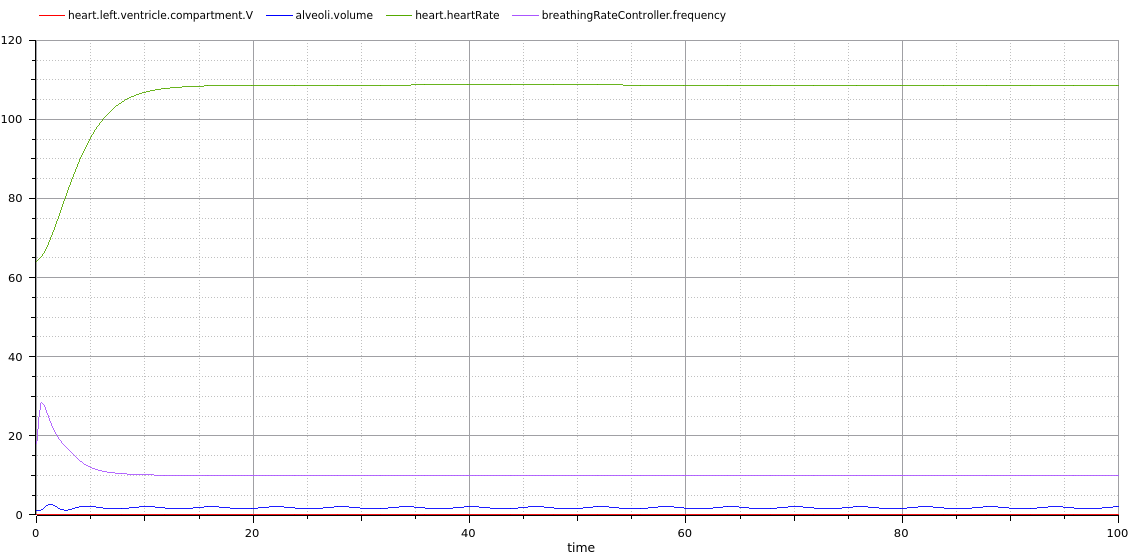
\includegraphics[scale=0.45]{IdaCpp.png}\\
			\footnotesize(b) {\sf C++} compilation code using IDA\\

	\end{tabular}
\end{center}
\vspace{-0.5cm}

\caption{Numerical results of the (a) CVode and (b) IDA solvers in {\sf C++} for the VHM.} \label{Fig:2}
\end{figure}

{\footnotesize
\begin{thebibliography}{10}

\bibitem{CppRuntime}{\sc Franke R, Walther M, Worschech N, Braum W \& Bachmann B}, 2015, {\em Model-based control with FMI and a C++ runtime for Modelica}, Proceedings of the 11\textsuperscript{th} International Modelica Conference, Versailles, France, pp.~339--347.

\bibitem{OpenModelica} {\sc OpenModelica}, 2016, {\em Open Source Modelica Consortium}, [Online], Cited 15\textsuperscript{th} March 2016, Available from {\url{https://openmodelica.org/}}





\end{thebibliography}}


\end{document}